\chapter*{Scenario 3 and 4 of CARDIS '15 paper}\label{Appendix_scenario3_4_cardis2015}

\subsubsection{Scenario 3.}
Let  $\newTraceLength$ be now variable and let the other parameters be fixed as follows: $\nbAttackTraces = 100, N_z=200, \numPoI = 3996$. Looking at Fig.~\ref{fig:3}, we might observe that the standard PCA might actually well perform in SCA context if provided with a larger number of kept components; on the contrary, a little number of components suffices to the LDA. Finally, keeping more of the necessary components does not worsen the efficiency of the attack, which allows the attacker to choose $\newTraceLength$ as the maximum value supported by his computational means.

\begin{remark}
In our experiments the ELV selection method only slightly outperforms the IPR. Nevertheless, since it relies on more sound and more general observations, {\em i.e.} the maximization of explained variance concentrated into few points, it is likely to be more robust and less case-specific. For example, in Fig.~\ref{fig:notSSS} it can be remarked that while the class-oriented PCA + ELV line keeps constant on the value 0 of guessing entropy, the class-oriented PCA + IPR is sometimes higher than 0.
\end{remark}

\todo{Is the table with results overview interesting?}
%
%\medskip
%
%\medskip
%
%  \begin{minipage}[c]{\textwidth}
%  \hspace*{-3mm}
%  \begin{minipage}[c]{0.45\textwidth}
%    \centering
%    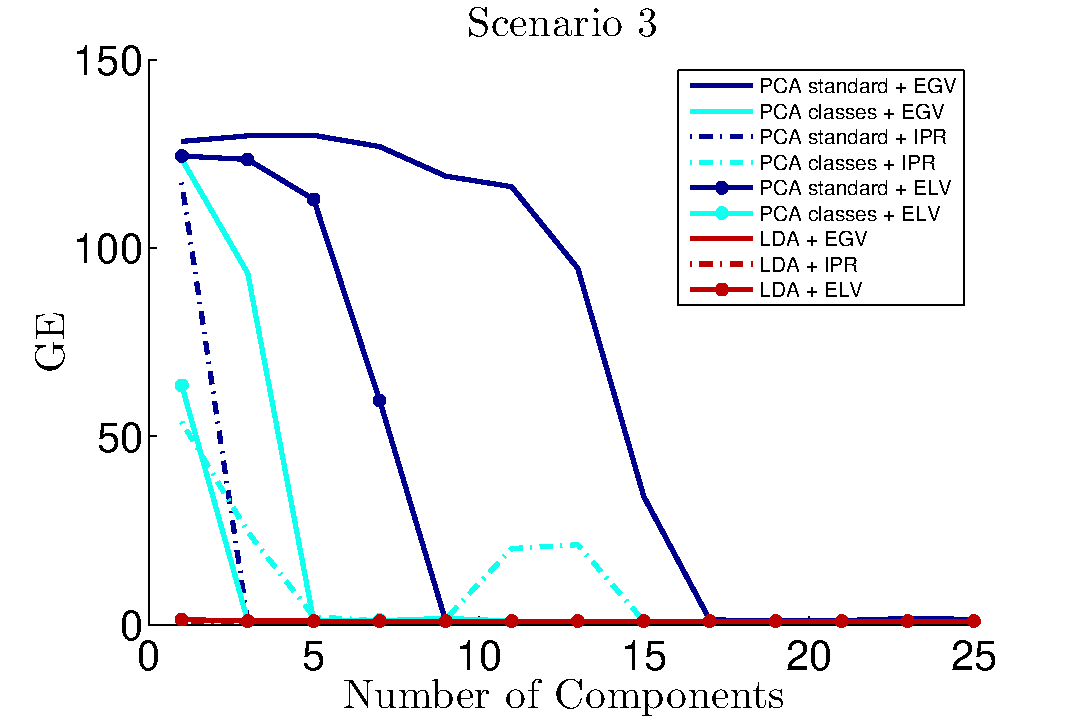
\includegraphics[width=\textwidth]{figures/Criterion3.pdf}
%    \captionof{figure}{Guessing Entropy as function of the number of the traces size after reduction}\label{fig:3}
%  \end{minipage}
%\hspace{1mm}
%  \begin{minipage}[c]{0.45\textwidth}
%    \centering
%    \begin{tiny}
%\begin{tabular}{|c|c|c|c|c|c|}
%\hline
%&&\multicolumn{4}{|>{\columncolor[gray]{0.7}}c|}{Parameter to minimize}\\
%\hline
%\multicolumn{1}{|>{\columncolor[gray]{0.7}}c|}{Method}&\multicolumn{1}{|>{\columncolor[gray]{0.7}}c|}{Selection}& $N$ &  $N'$ (SSS) &  $N'$ ($\neg$SSS) &  $C$ \\
%\hline
%PCA standard & EGV & {\bf -} &  &{\bf -} &{\bf -} \\
%\hline
%PCA standard &\multicolumn{1}{|>{\columncolor[gray]{0.8}}c|}{ELV} & \multicolumn{1}{|>{\columncolor[gray]{0.9}}c|}{{\bf -}} & &\multicolumn{1}{|>{\columncolor[gray]{0.9}}c|}{{\bf -}} &\multicolumn{1}{|>{\columncolor[gray]{0.9}}c|}{{\bf -}} \\
%\hline
%PCA standard & IPR &{\bf -} & &{\bf -} &{\bf +} \\
%\hline
%PCA class & EGV & {\bf -} &{\bf -} &{\bf -} &{\bf -} \\
%\hline
%PCA class & \multicolumn{1}{|>{\columncolor[gray]{0.8}}c|}{ELV} &\multicolumn{1}{|>{\columncolor[gray]{0.9}}c|}{{\bf +}} &\multicolumn{1}{|>{\columncolor[gray]{0.9}}c|}{$\bigstar$}&\multicolumn{1}{|>{\columncolor[gray]{0.9}}c|}{$\bigstar$} &\multicolumn{1}{|>{\columncolor[gray]{0.9}}c|}{{\bf +}} \\
%\hline 
%PCA class & IPR & {\bf {\bf +}} &$\bigstar$ &{\bf +} &{\bf -} \\
%\hline 
%LDA & EGV &$\bigstar$ & & {\bf +} & $\bigstar$\\
%\hline 
%LDA & \multicolumn{1}{|>{\columncolor[gray]{0.8}}c|}{ELV} & \multicolumn{1}{|>{\columncolor[gray]{0.9}}c|}{{\bf +}} &  & \multicolumn{1}{|>{\columncolor[gray]{0.9}}c|}{{\bf +}} & \multicolumn{1}{|>{\columncolor[gray]{0.9}}c|}{$\bigstar$}\\
%\hline 
%LDA & IPR & {\bf +} & &{\bf +} & $\bigstar$ \\
%
%\hline 
%\multicolumn{1}{|>{\columncolor[gray]{0.8}}c|}{$\SW$ Null Space}  & EGV & &\multicolumn{1}{|>{\columncolor[gray]{0.9}}c|}{$\bigstar$ } & & \\
%\hline 
%\multicolumn{1}{|>{\columncolor[gray]{0.8}}c|}{$\SW$ Null Space}  & IPR & &\multicolumn{1}{|>{\columncolor[gray]{0.9}}c|}{{\bf +}} & & \\
%\hline 
%\multicolumn{1}{|>{\columncolor[gray]{0.8}}c|}{Direct LDA} & EGV & & \multicolumn{1}{|>{\columncolor[gray]{0.9}}c|}{$\bigstar$}& & \\
%\hline 
%\multicolumn{1}{|>{\columncolor[gray]{0.8}}c|}{Direct LDA} & IPR & &\multicolumn{1}{|>{\columncolor[gray]{0.9}}c|}{{\bf +}}& & \\
%\hline
%\multicolumn{2}{|>{\columncolor[gray]{0.8}}c|}{Fisherface} & &\multicolumn{1}{|>{\columncolor[gray]{0.9}}c|}{{\bf -}} & & \\
%\hline 
%\multicolumn{2}{|>{\columncolor[gray]{0.8}}c|}{$\ST$ Spanned Space}  & &\multicolumn{1}{|>{\columncolor[gray]{0.9}}c|}{{\bf -}} & & \\
%\hline
%\end{tabular}
%\end{tiny}
%\captionof{table}{Overview of extractors performances in tested situations.}\label{table:results}
%    \end{minipage}
%  \end{minipage}
%
%\begin{figure}
%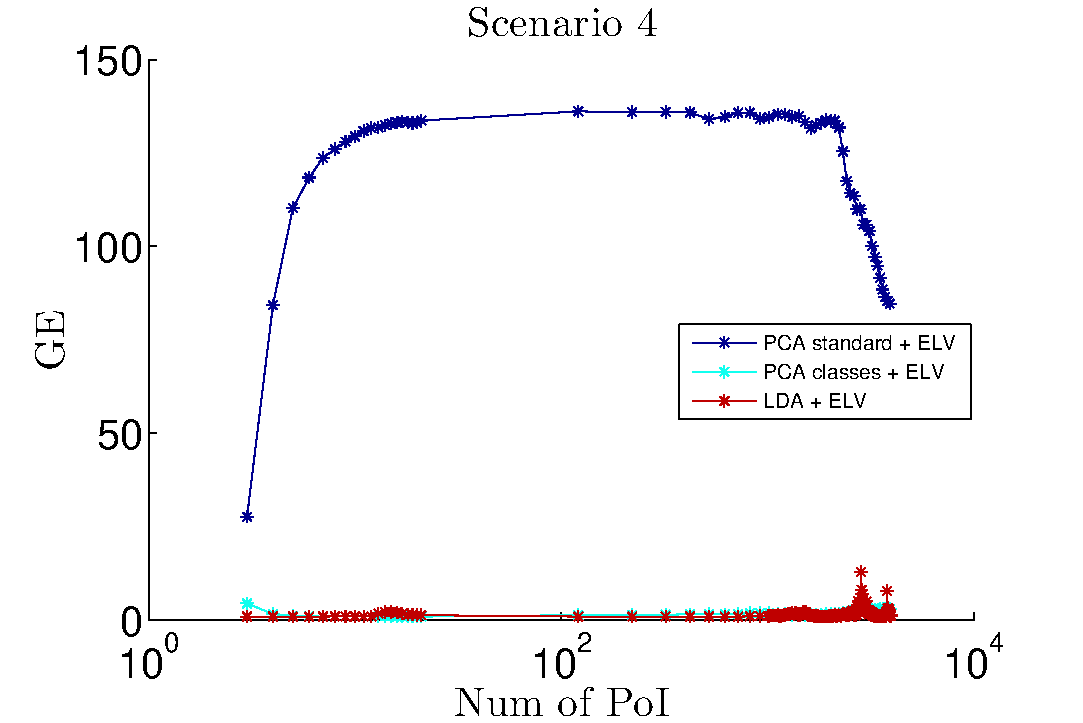
\includegraphics[width=0.5\textwidth]{figures/Criterion4.pdf}
%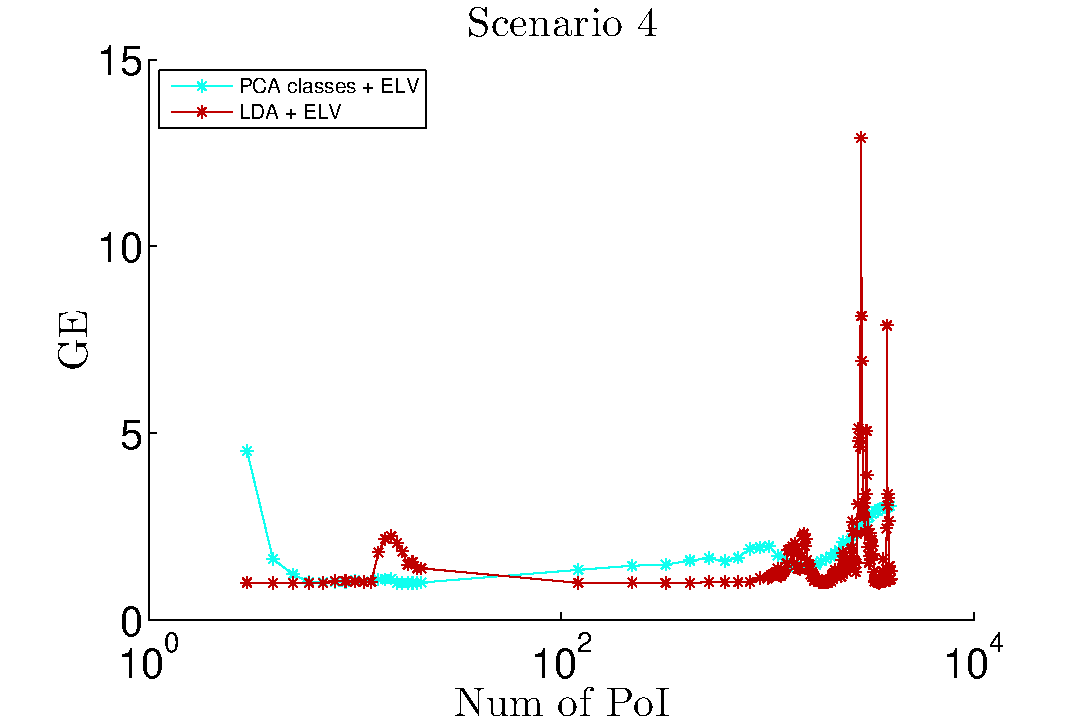
\includegraphics[width=0.5\textwidth]{figures/Criterion4cutted.pdf} 
%\caption{Guessing Entropy as function of the number of time samples contributing to the extractor computation.}\label{fig:4}
%\end{figure}
%
%An overview of the results of our comparison in scenarios 1, 2 and 3 is depicted in Table~\ref{table:results}: depending on the adversary purpose, given by the parameter to minimize, a $\bigstar$ denotes the best method, a ${\bf +}$ denotes a method with performances close to those of the best one and a ${\bf -}$ is for methods that show lower performances. Techniques introduced in this paper are highlighted by a grey background.  For example we remark that the class-oriented PCA takes advantage of the association with our ELV selection of components, achieving optimal performances when the goal is to minimize the number of profiling traces $\numTraces[]'$. As expected, when there are no constraints over $\numTraces[]'$, the LDA outperforms the other methods; however, even in this case which is very favourable to the LDA, the class-oriented PCA equipped with the ELV selection has an efficiency which is close to that of the LDA.
%


\subsubsection{Scenario 4.}


This is the single scenario in which we allow the ELV selection method to not only select the components to keep but also to modify them, keeping only some coefficients within each component, setting the other ones to zero. We select pairs \textit{(component, time sample)} in decreasing order of the ELV values, allowing the presence of only $\newTraceLength = 3$ components and $\numPoI$ different times samples: {\em i.e.}, we impose that the matrix $A$ defining the extractor (see \eqref{eq:linearExtractor}) has $\newTraceLength = 3$ rows (storing the 3 chosen components, transposed) and exactly $\numPoI$ non-zero columns.
Looking at Fig.~\ref{fig:4} we might observe that the LDA allows to achieve the maximal guessing entropy with only 1 PoI in each of the 3 selected components. 
Actually, adding PoIs worsen its performances, which is coherent with the assumption that the vulnerable information leaks in only a few points. Such points are excellently detected by the LDA. Adding contribution from other points raises the noise, which is then compensated by the contributions of further noisy points, in a very delicate balance. Such a behaviour is clearly visible in standard PCA case: the first 10 points considered raise the level of noise, that is then balanced by the last 1000 points.

